\chapter{Experiments and results}
We have shown that gossip transparency and the enforcement of exchange policies offer great potential
to defend against manipulators and free-riders. We implemented both mechanisms and establish in this chapter
how a practical system responds to manipulation attempts. More specifically we emulate honest agents,
manipulators and free-riders in small scale experiments. We can observe the behavior of the 
honest agents and find that strategic manipulators are detected and isolated. We show that honest agents who
execute our mechanism are able to effectively detect free-riding agents that do not share or do not verify their partners 
and ignore them for future interactions.

The rest of the chapter is structured as follows: we first give an overview of the software 
architecture. Then we explain the setup of the experiments and the types of strategic manipulation
that will be emulated. Finally we present the results of the experiments.

% In the previous chapters we have explored the problem of dissemination of information in distributed
% trust systems. We offered a solution in the form of our multichain based TrustChain architecture, extended 
% it with internal agent state transparency and designed a mechanism that prevents any free-riding on
% dissemination and validation of information on transactions. In this chapter we aim to prove the 
% properties of the mechanism and architecture by experimental analysis. We built a proof-of-concept
% software that fully implements the architecture and mechanism described in this work. It allows us 
% to run an emulation of an agent network and study the behavior of agents in the presence of strategic
% manipulators.

\section{Implementation details}
The experiments are run on a standalone implementation of TrustChain with the mentioned extension
and exchange mechanism. The code is available through GitHub\footnote{https://github.com/jangerritharms/aupair}.
The code is based on the TrustChain implementation of py-ipv8\footnote{https://github.com/tribler/py-ipv8}
another project that is developed in the context of BlockchainLab. 

The implementation is done in Python. The programming language was chosen as it allows for fast development,
offers many useful extensions and the py-ipv8 dependency is also written in Python. 

\begin{figure}[h!]
  \centering
  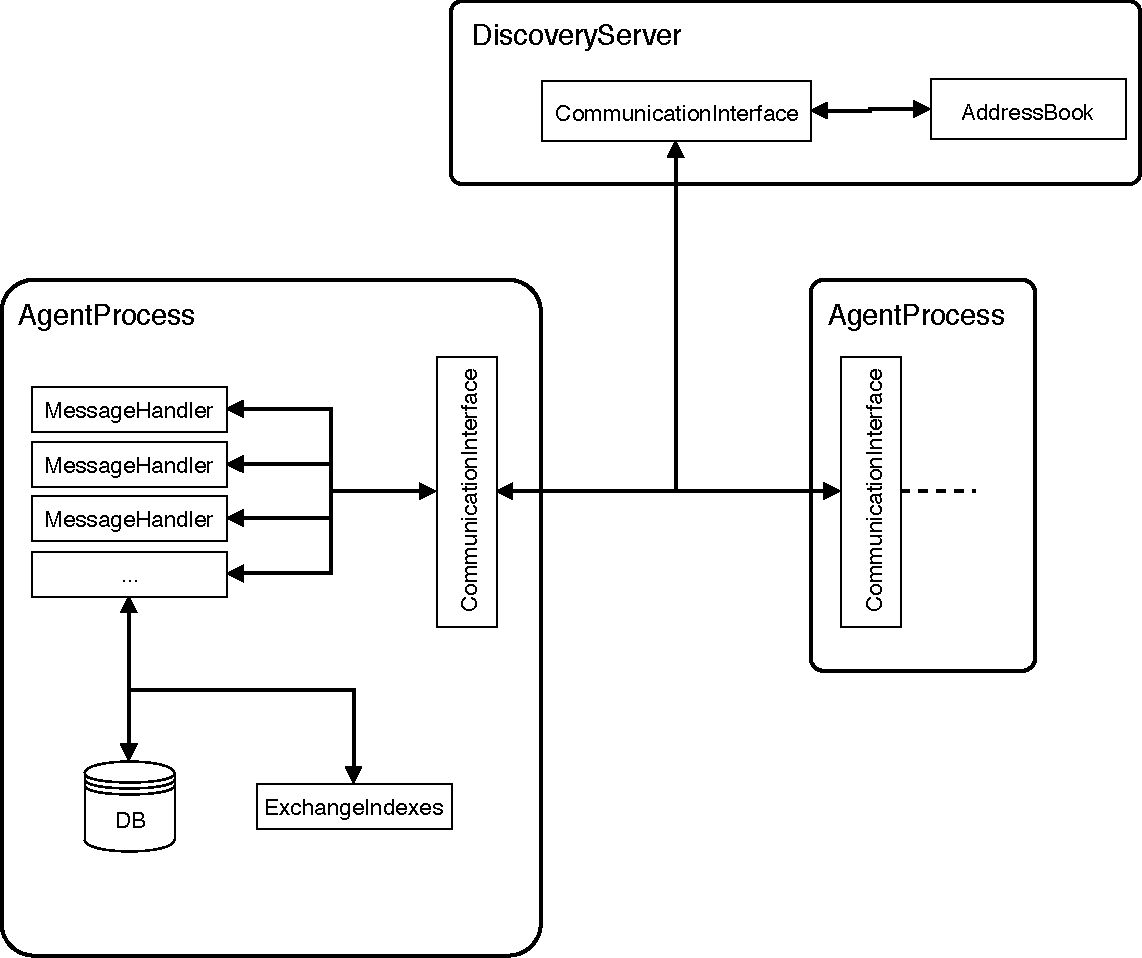
\includegraphics[width=\textwidth]{images/architecture.pdf}
  \caption{Architecture drawing of the experiment software.}
  \label{fig:software_architecture}
\end{figure}

An overview of the architecture is given by the drawing in Figure \ref{fig:software_architecture}.
At the core of the software is the agent module which defines the functionality of an agent.
In the experiment, multiple agents will be emulated. Each agent runs in a single process. Each agent 
has a communication interface. These interfaces connect and communicate with each other using tcp sockets, 
implemented using the \texttt{zeromq} library. Messages for the communication are defined in the 
Google \texttt{protobuf} format. Agents implement a set of message handlers which contain the main 
logic of the agents. In the experiment multiple types of agents will be emulated, each type of agent
reacts differently to the received messages. Each time an agent receives a message, the communication
interface will forward the message to the correct handler of the message based on the header of the 
message. Also each agent implements a MySQL database instance and a storage that map
the exchange blocks to the received blocks. Because each agent runs in an own process and acts on 
their own database, agents are completely independent, similar to a truly distributed network.
The basic TrustChain data structures and block database implementation were taken from the \texttt{py-ipv8} project. 

Next to the agents there is the discovery server which handles the peer discovery process. The 
experiment is started by spawning all agent processes and the discovery server. Once the agent 
process is started each agent sends a registering message to the discovery server to register the 
public key with the address of the tcp endpoint. After a 5 second initialization period it is assumed
that all processes have started and registered. The discovery server then sends a message to all 
registered agents containing their peers. Once that messages is received agents start running the
experiment. 

\section{Experiment design}
The goal of the experiments is to confirm our theoretical analysis of exchanges policies from Chapter 
\ref{chap:model} and our architecture in Chapter \ref{chap:implementation} in an experimental setup.
Four types of agent behavior will be analyzed in the experiments.

\begin{itemize}
    \item \textbf{Honest agent}: An agent that exchanges and verifies according to the Network-State-Exchange
    policy.
    \item \textbf{Exchange free-rider}: An agent that gains an advantage by not 
    expending resources on disseminating transaction records.
    \item \textbf{Verification free-rider}: An agent that gains an advantage by not expending 
    resources on verifying the behavior of their peers
    \item \textbf{Malicious}: An agent that manipulates or withholds information in order to gain an
    advantage. 
\end{itemize}

% The goal of the experimental analysis is to show that free-riding on dissemination and validation of
% transaction information is no longer possible with the extension of TrustChain proposed in 
% chapter~\ref{chap:state_transparency} and the mechanism in chapter~\ref{chap:mechanism}. This would
% be a major step towards a secure and valid distributed trust system. 

In the experiments we emulate small networks of up to 6 agents. All agents are trying to perform 
interactions with each other. The actual application domain is not modelled so transaction blocks 
are empty. Agents are acting completely autonomously but know about all the other agents in the network. 
At a frequency of 20 per second agents go through rounds, in each round an agent has a 1\% probability 
of starting an interaction. This adds up to approximately 1 transaction every 5 seconds. In addition 
agents respond to interaction requests from their peers asynchronously. 
At the start of the interaction a partner is selected with uniform probability from all connected peers. If an interaction with 
the selected partner is already ongoing, the new interaction request is cancelled without selecting a new partner. 

Once the interaction is started honest agents perform exchanges and verification according the 
mechanism as described in chapter \ref{chap:implementation}. The dishonest types of agents each have 
some deviation from the expected behavior in order to obtain an unfair advantage. 
All types of agents which were used in the experiments are listed in Table \ref{tab:agent_types}.
A more complete list of manipulators is discussed in Chapter \ref{chap:implementation}, however we 
implemented two types of manipulating behavior, block withholding and double spending.

\begin{table}
    \caption{Agent types used in the experiments}
    \label{tab:agent_types}
    \begin{tabular}{p{3cm}|p{3cm}|p{8cm}} \toprule
    \textbf{Type} & \textbf{Sub-type} & \textbf{Behavior} \\ \midrule
    \multirow{2}{3cm}{Honest agents} & without history check (default) & Exchanges and verifies agents normally \\ \cline{2-3}
    & with history check & additionally replays the history of a peer to find any deviating behavior in the past \\ \midrule
    \multirow{2}{3cm}{Exchange free-rider} & No exchanges & Does not create any exchanges \\ \cline{2-3}
    & Empty exchanges & Creates exchanges blocks with empty exchanges \\ 
    % & Self-requests & Exchanges only own chain \\ \hline
    \midrule
    Verification free-rider & - & Acts honestly but blindly trusts all partners without verifying their data or behavior \\ \midrule
    \multirow{2}{3cm}{Manipulator } & Block withholder & Creates a normal transaction and tries to hide it afterwards \\ \cline{2-3}
    & Double-spender & Creates two conflicting transactions and shares them with two different peers \\ \bottomrule
    \end{tabular}
\end{table}
    
With the experiments we study the behavior of honest agents in the presence of dishonest agents. If 
any agent fails a verification of an honest agent, that honest agent will subsequently ignore the 
dishonest agent. There is no forgiveness. However, honest agents do not communicate about any 
dishonest agents they discover.

\section{Experiment results}
In the following we will present the results of our experimental analysis.
\subsection{Dissemination free-riders}

% \begin{figure}
%     \centering
%     \begin{subfigure}{\textwidth}
%       \centering
%       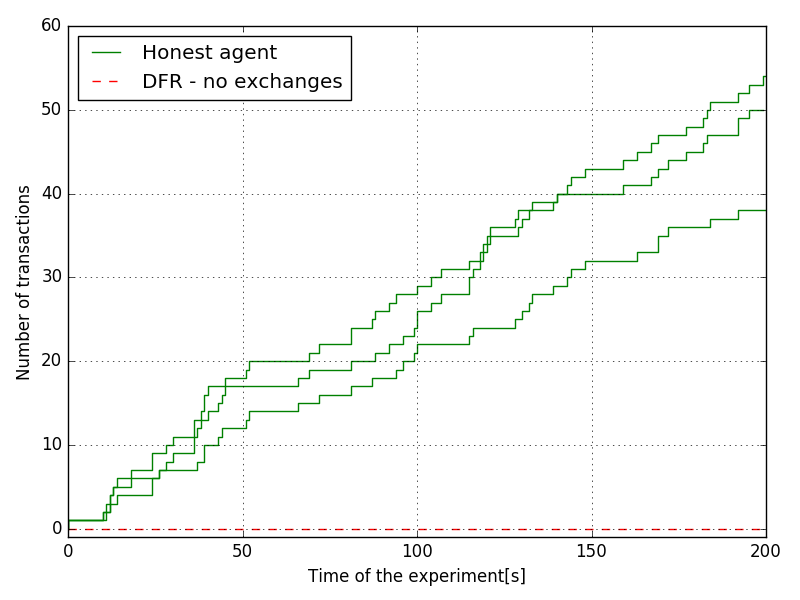
\includegraphics[width=.6\linewidth]{images/DFR_no_exchanges}
%       \caption{Transactions over time of honest agents with dissemination free-rider that does not 
%       perform any exchanges}
%       \label{fig:DFR_no_exchanges}
%     \end{subfigure}\\
%     \begin{subfigure}{\textwidth}
%       \centering
%       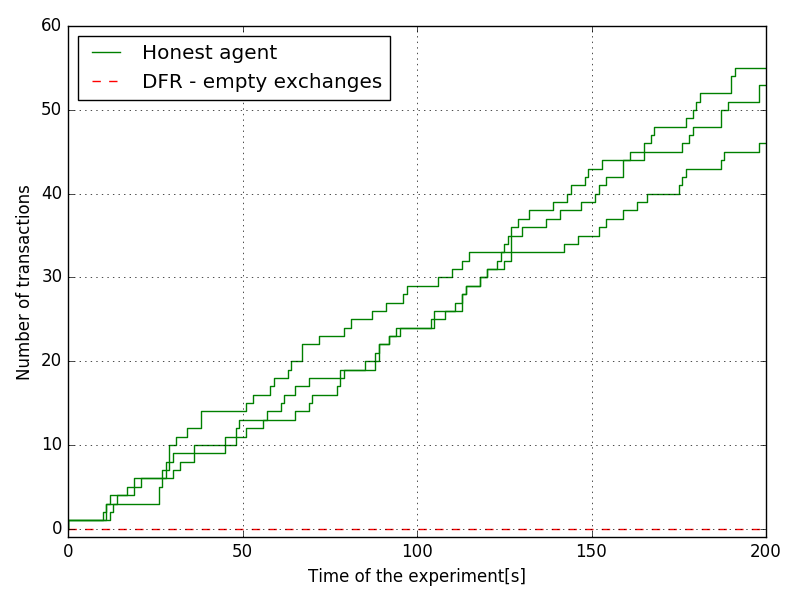
\includegraphics[width=.6\linewidth]{images/DFR_empty_exchanges}
%       \caption{Transactions over time of honest agents with dissemination free-rider that creates 
%       empty exchanges}
%       \label{fig:DFR_empty_exchanges}
%     \end{subfigure}\\
%     \begin{subfigure}{\textwidth}
%         \centering
%         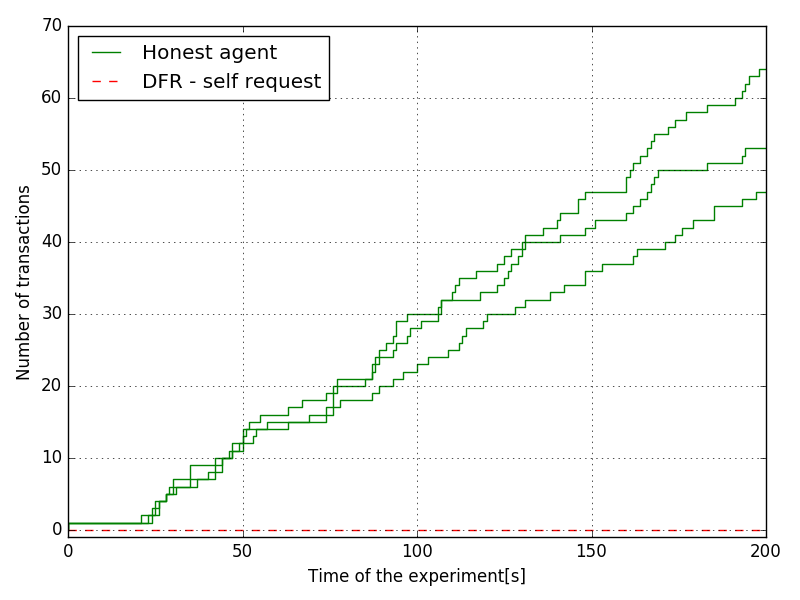
\includegraphics[width=.6\linewidth]{images/DFR_self_request}
%         \caption{Transactions over time of honest agents with dissemination free-rider that only 
%         exchanges own data}
%         \label{fig:DFR_self_request}
%       \end{subfigure}
%     \caption{Transactions over time of three experiments with different types of dissemination 
%     free-riders}
%     \label{fig:DFR}
% \end{figure}

\begin{figure}
  \centering
  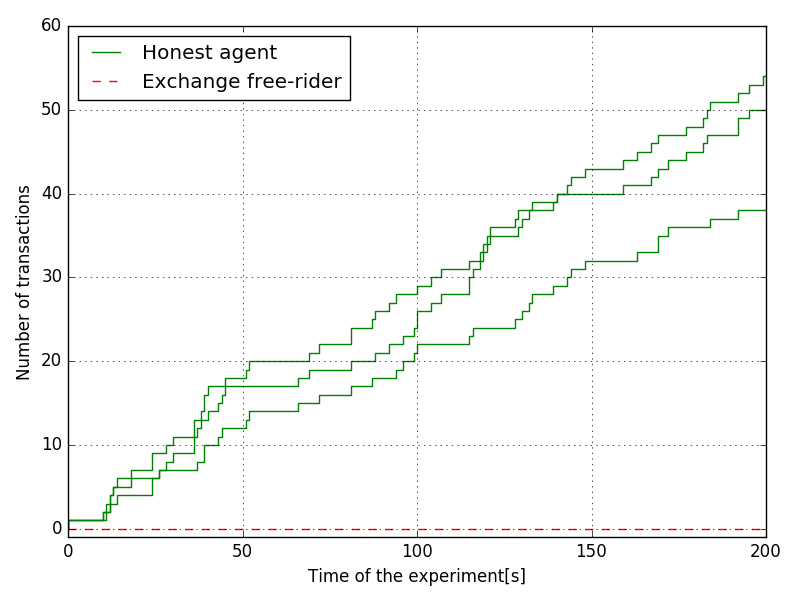
\includegraphics[width=.6\linewidth]{images/gossip_free-rider}
  \caption{Transactions over time of honest agents with exchange free-rider (both types give same result)}
  \label{fig:DFR_no_exchanges}
\end{figure}

Our first experiment analysis the performance of our exchange mechanism against free-riders. Gossip
free-riders that do not exchange information create a threat to the security of the network. In order
to secure the system, honest agents should be able to detect free-riders and ignore them. This will 
remove any possible future profit from free-riders which should incentivize them to become honest.

In this first set of experiments we observe the behavior of three honest agents in the presence of 
a exchange free-rider that performs no exchanges. Figure \ref{fig:DFR_no_exchanges} shows the number of transactions of each 
agent against the time of the experiment. All honest agents steadily increase their successful 
interactions throughout the experiment and end up between 40 to 60 transactions. The free-riding agent
is not able to perform a single interaction. That means all honest agents detected the free-rider 
as a dishonest agent and consequently ignored him. 

As expected, without gossiping an agent has no chance to interact with the honest agents. The 
experiment was repeated with the another type of exchange free-riders who is signing empty exchanges. 
The second experiment show the same outcome as in Figure \ref{fig:DFR_no_exchanges}:
the honest agents do not interact with the exchange free-riders.

The first type of free-riding agent does not exchange any data and therefore does not create any 
proof of exchanges. Also he is not willing to sign an exchange block that would document the acquisition
of foreign blocks. Yet in order to interact with honest agents the free-rider needs 
to publish a complete chain. Honest nodes detect the lack of exchange blocks upon inspection and 
subsequently distrust that agent. Because not even the first exchange block is signed, also the first
transaction is not completed as the honest agents only interact after a successful exchange.

The second type aims to create empty exchanges. In the role of the responder, the agent requests no 
blocks from the honest agents and as initiator the agent tries to claim that no blocks were received 
from the honest agent. However, by calculating 
that the free-rider should have requested blocks and by finding a wrong exchange hash in the other case
the honest agent can in both cases detect the fraud. That way, also in this case the honest agents 
are able to detect the wrong behavior.

% Finally, the third type of dissemination free-riders, results shown in Figure\ref{fig:DFR_self_request}
% , requests and sends data about itself but not any other knowledge. When in the responder position, 
% the agent can request only its own blocks. As initiator the agent tries to act again as if no data
% was received other than its own blocks. However the partner can see that the exchange block proposal
% does not properly represent the data exchanged and will therefore stop the transaction. Also this way
% the agent is not able to interact with honest partners. 

We find that dissemination free-riding leads to isolation and no transaction with honest partners. 
That means no reputation or trust will be build with this type of misbehaving agents and any hope for
future rewards is voided. Agents have to disseminate their data in order to be accepted and to prosper.

\subsection{Colluding free-riders}
Our second experiment analyses the impact of multiple free-riders in a collusion attack. In order to
be accepted as honest agents without gossiping, colluding agents can work together and sign empty exchanges for 
each other. This will create a seemingly valid history for the free-riders. Their goal is to interact 
with each other \textit{and} with the honest agents while exchanging less than data then necessary. Honest agents
should ignore them in order to keep their network safe and honest.

In order to analyze this situation we ran an experiment with three honest agents and three colluding gossip 
free-riders. The transactions are plotted against time in Figure \ref{fig:50percent}.

\begin{figure}[h!]
    \centering
    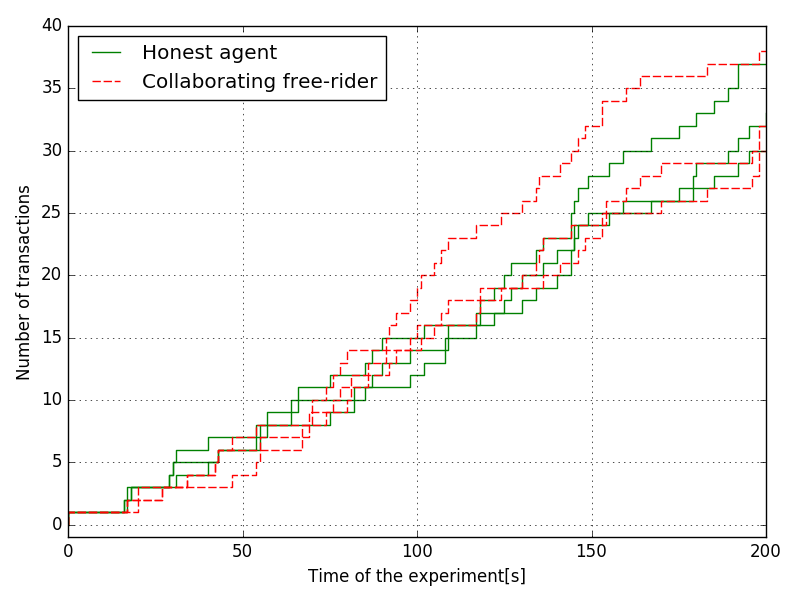
\includegraphics[width=0.7\textwidth]{images/50percent}
    \caption{Transaction history of three honest agents and three dissemination free-riders
    that are cooperating}
    \label{fig:50percent}
\end{figure}

\begin{figure}[h!]
    \centering
    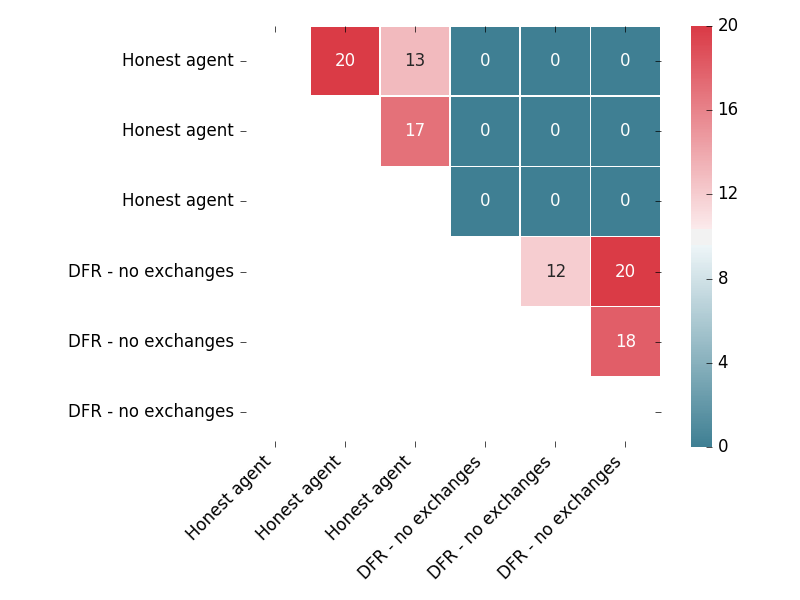
\includegraphics[width=0.8\textwidth]{images/50percent_interaction_matrix}
    \caption{Interaction matrix of quantifying the network separation}
    \label{fig:50percent_matrix}
\end{figure}

Again each line in the plot refers to the successful transactions of one agent. The plot shows six 
lines going almost in parallel which means that all agents fare equally well. However the plot does
not show which agents interact with each other. Therefore an interaction matrix is shown in Figure 
\ref{fig:50percent} which shows for each agent, how many interactions they had with each of their 
peers. 

From Figure \ref{fig:50percent_matrix} it becomes clear that no interactions (red squares) happen 
between honest and dishonest agents. Honest agents interact with honest agents, while dishonest
agents interact with dishonest agents. When dishonest agents try to interact with honest agents, 
honest agents will not sign an exchange block with empty hashes. So even though their history is 
correct according to the exchange policy, honest agents are still able to separate dishonest from
honest agents. This leads to network separation.

\subsection{Malicious behavior}
In the next experiment two types of malicious behaviors are analyzed: forking and block withholding. 
Similar to the free-riding, honest agents who use the TrustChain architecture and our exchange and 
verification mechanism should isolate the malicious agents. The results of the experiments are 
presented in a similar format as previously in Figure \ref{fig:malicious}.

Both agents perform an attack with a 25\% chance in each round.
The transaction hider is able to obtain six successful interactions before all honest agents ignore him and the line flattens. When trying to withhold a block any honest agent is able to detect the fraud. The agent is not able to hide any transactions because any future partner expects the complete chain from that agent. Any missing blocks in the chain will be seen as a manipulation attempt.

The same can be observed for the double-spender. After the fork happens, the forking agent is detected by a partner 
once the partner receives the two conflicting blocks. Depending on the peer selection and the network size, this can 
take several rounds. Therefore the forking agent is able to perform 9 interactions in the first 20 
seconds of the experiment. After those interactions the red line indicating the forking agent 
flattens, meaning no more successful interactions happen. 

\begin{figure}
    \begin{subfigure}{\textwidth}
      \centering
      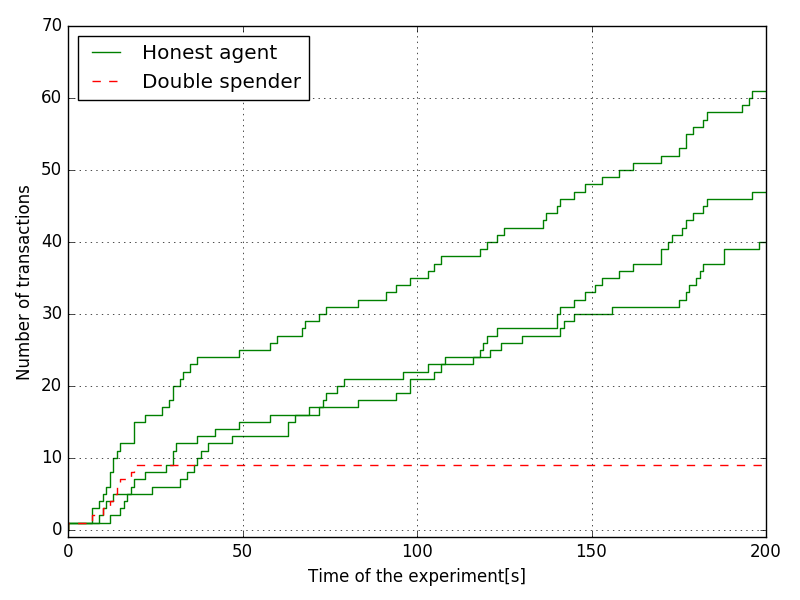
\includegraphics[width=.7\linewidth]{images/double_spending}
      \caption{Transaction history of three honest agents interacting with one strategic manipulator who performs a fork}
      \label{fig:forking}
    \end{subfigure}\\
    \begin{subfigure}{\textwidth}
      \centering
      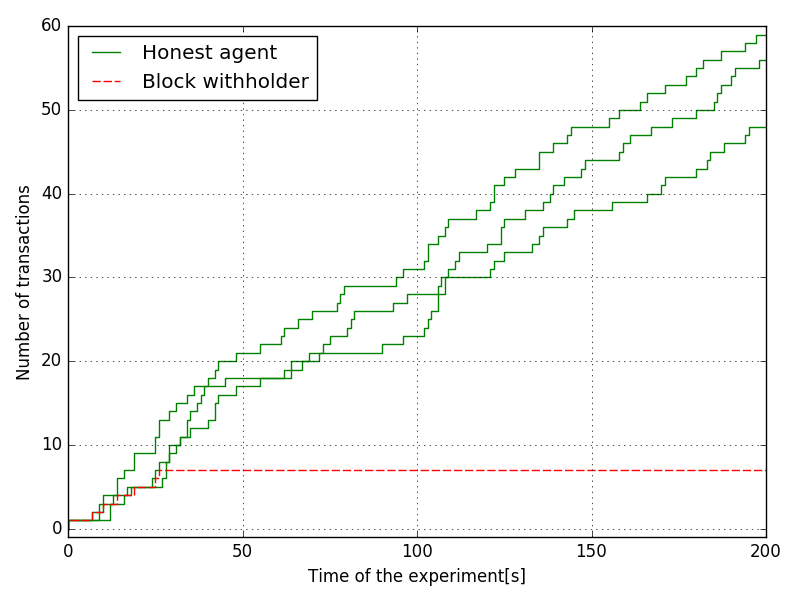
\includegraphics[width=.7\linewidth]{images/transaction_hiding}
      \caption{Transactions over time of three honest agents with one strategic manipulator who tries to hide a transaction}
      \label{fig:DFR_empty_exchanges}
    \end{subfigure}\\
    \caption{Experiments of honest agents with sinlge malicious agents}
    \label{fig:malicious}
\end{figure}

\subsection{Verification free-rider}
In the previous experiment we showed that malicious agents can be detected and isolated. In Chapter
\ref{chap:model} we have presented a theoretical study that shows that with the Network-State-Exchange
policy also those agents that knowingly interact with those malicious agents can
be isolated. This is possible be ``replaying'' the complete history of an agent and redoing the 
verifications. Any honest agent that obtains the full knowledge of the subject can perform this check 
ad find any failing verification which signals dishonest behavior.

We first show how three honest agents who do not perform the history verification act in the 
presence of one malicious agent and one verification free-rider. This is to show that without the 
history replay an agent that knowingly interacts with a malicious agent cannot be detected. In such 
a situation the verification free-rider performs a successful attack.

The results are presented in Figure \ref{fig:verification_doublespend_honest_combined}. As expected,
the verification free-rider, represented by the blue dotted line in the figure is able to perform 
just as well as the honest agents. The forking agent is mostly ignored. The interaction matrix in 
Figure \ref{fig:verification_doublespend_honest_matrix} shows that most of the interactions of the 
forking agent come from the verification free-rider who does not perform any checks and therefore 
does not care about the fork.

\begin{figure}[h!]
    \begin{subfigure}{\textwidth}
      \centering
      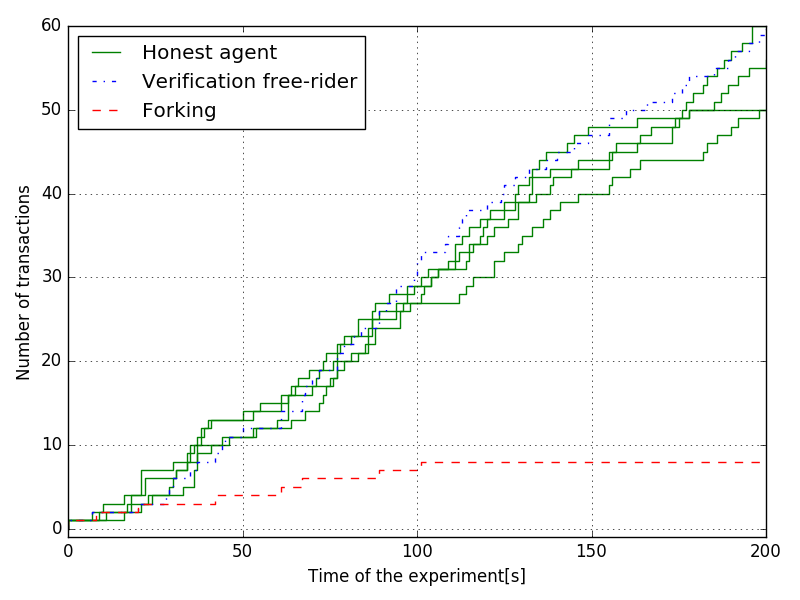
\includegraphics[width=.7\linewidth]{images/verification_doublespend_honest}
      \caption{Transaction history of three honest agents interacting with one strategic manipulator who performs a fork and a verification free-rider}
      \label{fig:verification_doublespend_honest}
    \end{subfigure}\\
    \begin{subfigure}{\textwidth}
      \centering
      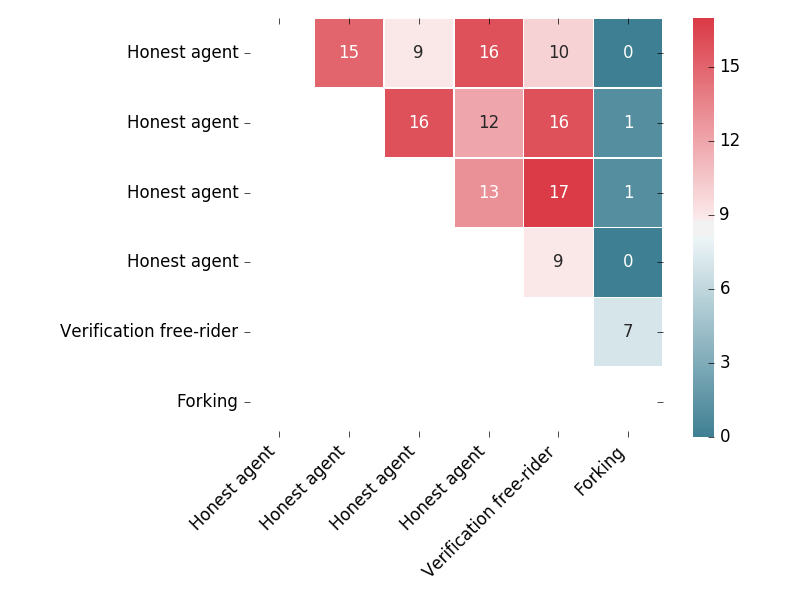
\includegraphics[width=1\textwidth]{images/verification_doublespend_honest_matrix}
      \caption{Interaction matrix of three honest agents with one strategic manipulator who performs a fork and a verification free-rider}
      \label{fig:verification_doublespend_honest_matrix}
    \end{subfigure}\\
    \caption{Experiment with three honest agents without replay verification, one malicious agent 
    and one verification free-rider}
    \label{fig:verification_doublespend_honest_combined}
\end{figure}

Next we repeated the experiment, but this time the honest agents perform replay verification of their
partners before every interaction. The results are shown in Figure \ref{fig:verification_doublespend_combined}. 

The results show that after a long initial phase in which the blue and red curve seem to follow 
the green curves, they do get shallower after around 100seconds. It is quite obvious, at least 
from the 100 second mark onwards, that the blue and red curve are running exactly in parallel. This is
because after detecting the forking agent and the verification free-rider, the honest agents are 
able to identify \textit{both} dishonest agents and ignore them for future interactions. Also the interaction
matrix shows that in the end, both dishonest agents get few interaction with the honest agents. 

\begin{figure}[h!]
    \begin{subfigure}{\textwidth}
      \centering
      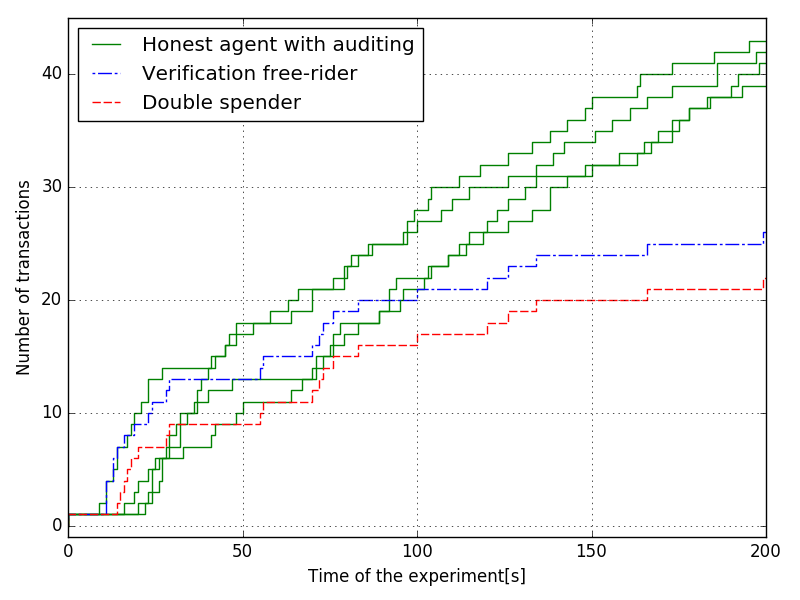
\includegraphics[width=.7\linewidth]{images/verification_doublespending}
      \caption{Transaction history of three honest agents with replay verification interacting with one strategic manipulator who performs a fork and a verification free-rider}
      \label{fig:verification_doublespending}
    \end{subfigure}\\
    \begin{subfigure}{\textwidth}
      \centering
      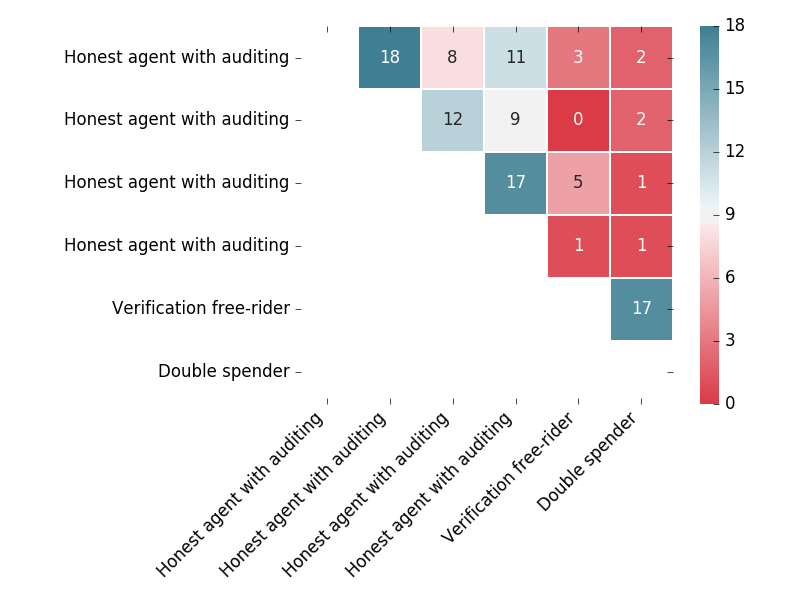
\includegraphics[width=.9\linewidth]{images/verification_doublespending_matrix}
      \caption{Interaction matrix of three honest agents with replay verification with one strategic manipulator who performs a fork and a verification free-rider}
      \label{fig:verification_doublespending_matrix}
    \end{subfigure}\\
    \caption{Experiment with three honest agents without replay verification, one malicious agent 
    and one verification free-rider}
    \label{fig:verification_doublespend_combined}
\end{figure}
